\documentclass{beamer}

%
% Elige el aspecto de su presentación.
% Para más temas, temas de color y fuentes, consulta:
% http://deic.uab.es/~iblanes/beamer_gallery/index_by_theme.html
%
\mode<presentation>
{
  \usetheme{Warsaw}       % o prueba Darmstadt, Madrid, Dresden, ...
  \usecolortheme{default} % o prueba albatross, beaver, crane, ...
  \usefonttheme{default}  % o prueba serif, structurebold, ...
  \setbeamertemplate{navigation symbols}{}
  \setbeamertemplate{caption}[numbered]
} 

\usepackage[spanish]{babel}
\usepackage[utf8]{inputenc}
\usepackage{amsmath}

\title{Las cuentas del Gran Capitán}
\author{Perico de los Palotes}
\institute{Reino de Castilla y León}
\date{\today}

\begin{document}

\begin{frame}
  \titlepage
\end{frame}

\begin{frame}{Guión}
  \tableofcontents
\end{frame}

\section{Orden del día}

\begin{frame}{Orden del día}

\begin{itemize}
  \item Objetivos
  \item Descripción general
  \item Realización
\end{itemize}

\end{frame}

\begin{frame}{¡Fuera del orden del día!}

\begin{itemize}[<+->]
  \item Picos, palas y azadones, cien millones de ducados
  \item Frailes, monjas y pobres, ciento cincuenta mil ducados
  \item Guantes perfumados, cien mil ducados
  \item Reponer y arreglar las campanas, ciento sesenta mil ducados
  \item Pequeñeces del rey, cien millones de ducados 
\end{itemize}

\end{frame}

\section{Antecedentes}

\begin{frame} {Objetivos clave y  factores de éxito}

\begin{itemize}
\item Campaña de Nápoles
  \begin{itemize}
    \item Conquistar el reino de Nápoles
    \item Ganar acceso al resto de Italia
  \end{itemize}
\end{itemize}

\begin{block}{Visión compartida}
\begin{itemize}
\item La victoria ha sido total
\item Los  recursos concedidos han sido escasos
\end{itemize}
\end{block}

\end{frame}

\section{Descripción general}

\begin{frame}{Descripción general}

\begin{figure}
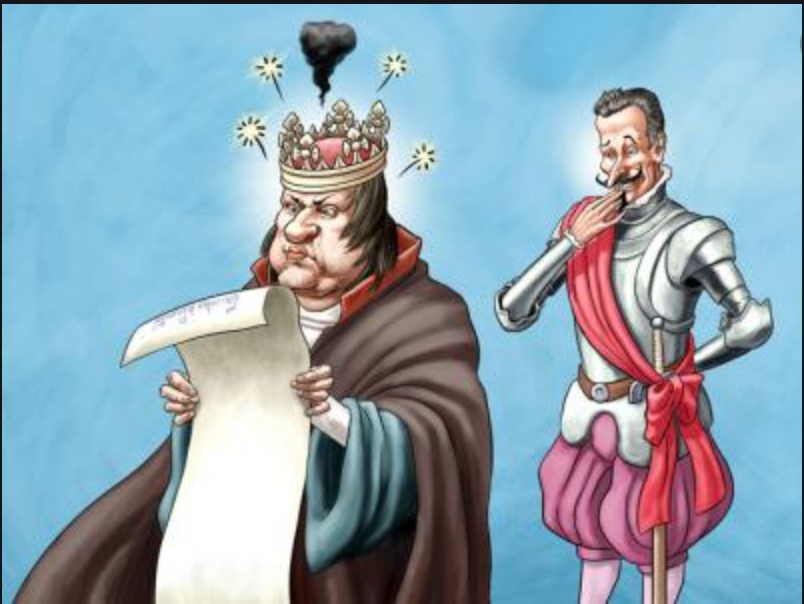
\includegraphics[width=0.4\textwidth]{cuentas}
\end{figure}

\begin{center}
{\scriptsize
\begin{tabular}{|l|r||r|}
\hline
Concepto & Coste & Coste acumulado \\
\hline
\hline
Picos, \ldots & 100.000 K & 100.000 K\\
\hline
Frailes, \ldots & 150 K & 100.150 K \\
\hline
Guantes \ldots & 100 K & 100.250 K \\
\hline
Campanas \ldots & 160 K & 100.410 K \\
\hline
Pequeñeces \ldots  & 100.000 K & 200.410 K \\
\hline
\end{tabular}}
\end{center}

%\begin{block}{Un intermedio matemático}
%\begin{equation*}
%g(x)=\begin{cases}
%sin(x), \text{ si } x \in [0,\pi]; \\
%cos(-x), \text{ si } x \in [\pi,2\pi].
%\end{cases}
%\end{equation*}
%\end{block}

\end{frame}

\section{Conclusiones}

\begin{frame}{Conclusiones}

\begin{columns}
\begin{column}{0.4\textwidth}
\begin{itemize}
\item Hemos ganado la guerra
\item Sin apenas tropas
\item Con un presupuesto reducido
\end{itemize}
\end{column}
\begin{column}{0.6\textwidth}
\begin{itemize}
\item Los soldados han mostrado arrojo y generosidad
\item Han regalado un reino a España
\item No se merecen estas pequeñeces
\end{itemize}
\end{column}
\end{columns}

\end{frame}

\end{document}

